\documentclass[12pt]{article}
\usepackage{amsmath}
\usepackage{graphicx,psfrag,epsf,float, bm}
\graphicspath{C:/Users/Colin/Documents/GitHub/BB_data_analysis/paper/fig/}
\usepackage{enumerate}
\usepackage[numbers]{natbib}
\usepackage{url} % not crucial - just used below for the URL


\usepackage[x11names]{xcolor}
\usepackage{framed} % provides framed env., should be removed in final draft
\definecolor{shadecolor}{rgb}{1,.5,.5}

% math macros 

\newcommand{\ind}{\stackrel{ind.}{\sim}}
\newcommand{\op}{\operatorname}

\newcommand{\myequation}{\begin{equation}}
\newcommand{\myendequation}{\end{equation}}
\let\[\myequation
\let\]\myendequation


\pdfminorversion=4
% NOTE: To produce blinded version, replace "0" with "1" below.
\newcommand{\blind}{0}

% DON'T change margins - should be 1 inch all around.
\addtolength{\oddsidemargin}{-.5in}%
\addtolength{\evensidemargin}{-.5in}%
\addtolength{\textwidth}{1in}%
\addtolength{\textheight}{1.3in}%
\addtolength{\topmargin}{-.8in}%


\begin{document}

\def\spacingset#1{\renewcommand{\baselinestretch}%
{#1}\small\normalsize} \spacingset{1}


%%%%%%%%%%%%%%%%%%%%%%%%%%%%%%%%%%%%%%%%%%%%%%%%%%%%%%%%%%%%%%%%%%%%%%%%%%%%%%

\if0\blind
{
  \title{\bf A Hierarchical Bayesian Approach for Modeling Infant-Mortality and Wearout Failure Modes}
  \author{Eric Mittman\thanks{
    The authors gratefully acknowledge Bill Meeker for his comments and suggestions}\hspace{.2cm}\\
    Department of Statistics, Iowa State University\\
    and \\
    Colin Lewis-Beck \\
    Department of Statistics, Iowa State University}
  \maketitle
} \fi

\if1\blind
{
  \bigskip
  \bigskip
  \bigskip
  \begin{center}
    {\LARGE\bf Title}
\end{center}
  \medskip
} \fi

\bigskip
\begin{abstract}
% Consumers have an interest in accurate assessment of product reliability.  However, lifetime data is often sparse and has limited information.  
While reliability is an important aspect of product quality, by its nature, the lifetime data available to consumers tends to be limited; high-reliability consumer products fail infrequently. Due in part to multiple causes of failure, simple parametric models have limited application, being unable to capture relevant lifetime characteristics. On the other hand, more suitable models are difficult to fit because of small sample sizes. If it were available, failure analysis could mitigate identifiability issues; however, consumers do not have this information, nor is it have practical value for them.

In this paper we present a method for joint estimation of multiple lifetime distributions based on the Generalized Limited Failure Population (GLFP) model \citep{chan}. This 5-parameter model for lifetime data accommodates lifetime distributions with multiple failure modes:  early failure due to "infant mortality" and failure due to wearout. We fit the GLFP model using a hierarchical Bayesian approach.  Borrowing strength across populations, our method enables estimation with uncertainty of lifetime distributions even in cases where the number of model parameters is larger than the number of observed failures.  Moreover, using a Bayesian approach, comparison of different product brands is straightforward as estimation of arbitrary functionals are easily computable from the full posterior distribution.
\end{abstract}

\noindent%
{\it Keywords:} GLFP, Bathtub hazard, Censored data, Hierarchical models, Bayesian estimation
\vfill

\newpage
\tableofcontents
\newpage
\spacingset{1.45} % DON'T change the spacing!
\section{Introduction}
Consumers have an interest in accurate assessment of product reliability. Toward this end, there is a need for models that can fit the data together with methods that account for uncertainty.  While computationally convenient, simple parametric models can fail to capture key characteristics found in real data.

In this paper we present a method for joint estimation of multiple lifetime distributions based on the GLFP model \citep{chan}. This 5-parameter model for lifetime data accommodates lifetime distributions displaying early failures due to "infant mortality" and wearout. By borrowing strength across populations, our method enables estimation with uncertainty of lifetime distributions even in cases where the number of model parameters is larger than the number of observed failures. By producing samples from the full posterior distribution, estimation of arbitrary functionals is straightforward.

We illustrate this method on hard drive reliability data from a cloud-based computing company.  The data contains both left-truncation and right-censoring.  Also, the information in the data is unevenly distributed across the populations of interest making a hierarchical approach especially advantageous. 

\subsection{Motivation}

Failure distributions of high-reliability consumer products can be difficult to assess.  Even when field data are available, information may be limited for a variety of reasons.  Certain brands may have few products in operation resulting in small sample sizes.  Other products could have many observed units in operation but few observed failures or limited time under observation, which makes fitting a parametric lifetime model problematic.  In this paper, we propose the use of Bayesian hierarchical modeling to borrow information across products, thereby improving inferences on lifetime distributions where information is limited by small sample sizes, left-truncation, and right censoring. 

The reliability of many engineered products follow a similar pattern. Relatively high rates of failure occurring in early life ("infant mortality") due to defects from the manufacturing process. After this "burn-in" period, failure rates stabilize as the majority of defective units have failed and are no longer in the population.  Finally, after prolonged use, rates of failure increase due to wearout.  Ignoring this pattern in failure rates can lead to suboptimal decisions and spurious inferences about a product's reliability.   While simple nonparametric methods are available, such as the Kaplan-Meier estimator, these are not suitable for forecasting.  They also do not allow for a straight forward statistical comparisons of different brands in order to select the most reliable product. 

For real reliability data, often no failure analysis is available allowing objective discernment about when a failure is due to infant mortality. This presents a dilemma for analysts: the data may indicate more than one failure mode, contraindicating the use of a unimodal parametric distribution. However, without any knowledge of cause of failure, traditional competing risk models are not identifiable. \citet{chan} proposed the Generalized Limited Failure Population (GLFP) model. This model can provide a solution to the problem of unknown cause of failure (masking) in the special case where there is evidence of two modes of failure which impact different stages of product life. It avoids non-identifiability by introducing a parameter representing the population proportion defective. Where this parameter is zero, the GLFP model reduces to a unimodal distribution. \\

While the GLFP model provides flexibility and accords with a macro-level theory of product failure, it requires a lot of data to fit because of its complexity. Bayesian methods offer a means of reducing the amount of data required to fit the model by leveraging multiple sources of information. When multiple populations are of interest, comparisons based on separate, unrestricted GLFP model fits will be limited to those products with sufficient data. As we will show, hierarchical modeling of the GLFP parameters allows for borrowing of information across populations, imposing "soft" constraints on model parameters. This enables estimation for all product groups.  Populations with lots of data will be precisely estimated.  For products with limited data the posterior distribution of time-to-failure will contain greater uncertainty, while being shrunk toward a "pooled" model. Finally, in order to compare the reliability across brands, the Bayesian approach is appealing as samples obtained from the posterior distribution via Markov Chain Monte Carlo allow for easy numerical integration for computing  various quantities of interest. \\

% the model captures drive-models with lots of observed failures, while the predicted time to failure for drive-models with less information is over or under estimated. 

%\begin{shaded}
  %THIS SHOULD BE SEPARATED OUT
  %At the other extreme, separately fitting the model to each drive-model, is difficult for drive-models where the data are not strongly informative.  Due to identifiability issues, in these cases the model fit is unstable unless strongly informative priors are chosen.  \\
  %
  %We therefore propose to fit the GLFP model using a hierarchical Bayesian approach.  With over 60 drive-models in operation, a hierarchical model is advantageous as allows for borrowing of information to improve estimation of the GLFP parameters for each drive-model.  Moreover, the hierarchical model is a nice compromise between the aggregate and individual modeling approaches: drive-models with lots of failures are estimated precisely; and in cases where little data is available the hierarchical model borrows information from other drive-models to obtain stable estimates.  This allows us to include more of the hard drive data and more importantly, make valid inferences for each group of hard drive brands.\\
  %
  %
  %Failure data for series systems may be collected at the system level
  %by end-users interested only in the lifetime of the system. \citet{chan} proposed the generalized limited failure population
  %model (GLFP), for
  %failure times in a population where some units are susceptible to infant mortality. This model
  %covers a subset of the class of distributions known as bathtub distributions
  %\cite{sujata}. Bathtub distributions are characterized by a U-shaped
  %hazard function, where early failures are due to infant mortality and
  %late failure are due to wearout. While complex systems actually
  %exhibit more than two modes of failure, suitable parametric models
  %which can suitably approximate the overall lifetime distribution are
  %useful. 
  %
  %In the case of complex, high-reliability systems where cause of failure is
  %not available, a model which
  %\begin{enumerate}[a.]
  %\item has parameters that can be estimated from the observed data
  %\item is flexible enough to fit the observed data
  %\item in interpretable with respect to available theory of the underlying process
  %\end{enumerate}
  %is desired. We present a Bayesian, hierarchical modeling approach for
  %grouped failure data. As a benefit of working with Monte Carlo
  %samples, we can easily make inference on a wide range of quantities of
  %interest while accounting for uncertainty. We demonstrate this approach on real data hard
  %drive failure data from a
  %cloud-based storage company.
%\end{shaded}
%
%To model this mixture of failure distributions in a unified framework, Chan and Meeker proposed the Generalized Limited Failure Population (GLFP) model \citet{chan}.  In addition to describing the failure time distribution for products that are susceptible to infant mortality and wearout failure modes, it theorizes an unknown proportion of defective units which are susceptible to defects.    While the GLFP model provides flexibility over a simple or piece-wise parametric model, it can be difficult to fit with limited data  As Chan and Meeker discuss in their original paper, few observed failures in addition to unknown causes of failure cause maximum likelihood estimates to be unstable or impossible to obtain.  Therefore, when multiple populations are of interest, comparisons based on the standard GLFP model are restricted to those with sufficient data and observed failure from each failure mode.  A naive approach to this limitation is to combine the data from all products and fit a single GLFP model.  This model can be well-estimated, but the pooled GLFP model fits poorly.  At the other extreme, fitting a separate GLFP model to each product is problematic for products where the data are weakly informative.  Due to identifiability issues, in these cases the model fit is unstable unless strongly informative priors are placed on the model parameters.  \\
%
%We therefore propose to fit the GLFP model using a hierarchical Bayesian approach.  A hierarchical model is advantageous as allows for borrowing of information to improve estimation of the GLFP parameters for a whole class of products.  Moreover, the hierarchical model is a nice compromise between the aggregate and individual modeling approaches: product brands with lots of failures are estimated precisely; and in cases where little data is available the hierarchical model borrows information from other products to obtain stable estimates.  This allows us to include all of the data and more importantly, make valid inferences for each individual product.
%
%
%Failure data for series systems may be collected at the system level
%by end-users interested only in the lifetime of the system. \citet{chan} proposed the generalized limited failure population
%model (GLFP), for
%failure times in a population where some units are susceptible to infant mortality. This model
%covers a subset of the class of distributions known as bathtub distributions
%\cite{sujata}. Bathtub distributions are characterized by a U-shaped
%hazard function, where early failures are due to infant mortality and
%late failure are due to wearout. While complex systems actually
%exhibit more than two modes of failure, suitable parametric models
%which can suitably approximate the overall lifetime distribution are
%useful. 
%
%In the case of complex, high-reliability systems where cause of failure is
%not available, a model which
%\begin{enumerate}[a.]
%\item has parameters that can be estimated from the observed data
%\item is flexible enough to fit the observed data
%\item in interpretable with respect to available theory of the underlying process
%\end{enumerate}
%is desired. We present a Bayesian, hierarchical modeling approach for
%grouped failure data. As a benefit of working with Monte Carlo
%samples, we can easily make inference on a wide range of quantities of
%interest while accounting for uncertainty. We demonstrate this approach on real data hard
%drive failure data from a
%cloud-based storage company.

\subsection{Overview}
The structure of the paper is as follows.  Section~\ref{sec:Background} describes some of the potential applications of our method and summarizes previous related work found in the literature. Section~\ref{sec:GLFP model} introduces the GLFP model and illustrates an application in an example. Section~\ref{sec:Hierarchical GLFP model} introduces a hierarchical model for extending the GLFP model to multiple populations. In section~\ref{sec:Data analysis} we illustrate applying the hierarchical GLFP model to a real data set. Subsection~\ref{sec:Data} describes and summarizes the Backblaze Hard Drive data set.  Subsection~\ref{sec:Model Comparisons} shows the use of approximate leave-one-out cross-validation as a way to do model selection between different hierarchical model specifications. We also address computational issues and modeling decisions that lead to a final model.  In subsection~\ref{sec:Drive-model Comparisons} we present an analysis comparing drive-model lifetime distributions.  Finally, in section~\ref{sec:Conclusions}, we discuss the strengths and limitations of our method and consider extensions and alternatives.

\section{Background}
\label{sec:Background}
In engineering applications, a product can often fail from one out of a set of possible malfunctioning components.  For example, a computer system can break if the mother board, disc drive or power supply stop working.  Circuit boards (CB) can fail due to a manufacturing defect or later as a result of wearout.  The general name for such products is a series system where the lifetime of the product is the minimum failure time across $s$ different components or risks \cite{nelson}.  A common assumption in series systems is the time to failure for each risk, $s$, is statistically independent.  Thus, the overall reliability of a unit is modeled using the product rule across all $s$ risks.  Parameter estimation is straightforward if the cause of failure is known for each observation.  With engineering systems data, however, the exact cause of failure is frequently unknown or masked from the analyst.  \\

Previous papers have employed various data assumptions and methodologies to model masked lifetime failure data.  When modeling computer system failures Reiser et al. assumed each observed failure came from a known subset of failure modes, and estimation was performed using a Bayesian approach \cite{reiser}.  Chan and Meeker labeled the cause of circuit board failures as infant mortality, unknown, or wearout based on the time of observed failures.  This helped identify parameters when using maximum likelihood (ML) estimation.  Extending Chan and Meeker's analysis, Basu et.al performed a Bayesian analysis with informative priors to better identify early versus late failure modes without making any data assumptions \cite{basu}.  Berger and Sun introduced the Poly-Weibull distribution where cause of failure is the minimum of a several Weibull distributions \cite{berger}.  More recently, Ranjan et al. considered a competing risk model for infant mortality and wearout as a mixture of Weibull and exponential failure distributions \cite{ranjan}.  Treating the unknown failure modes as incomplete data, an expectation maximization (EM) algorithm providing ML estimates was used, in addition to Bayesian estimation.


\section{Generalized Limited Failure Population model}
\label{sec:GLFP model}

\subsection{Weibull parameterization}
\label{sec:Weibull parameterization}
For a random variable $Y$ following a Weibull distribution, the standard parameterization of the cumulative distribution function, in terms of scale parameter $\alpha$ and shape parameter $\beta$, is

$$ P(Y \le y) = 1 - \exp \left\{ \left( \frac{y}{\alpha} \right)^\beta \right\}. $$

An alternative parameterization, in terms of log-location parameter $\mu = \log \alpha$ and log-scale parameter $\sigma = 1/\beta$ is

$$ P(Y \le y) = 1 - \exp \left\{ -\exp \left( \frac{ \log y - \mu }{\sigma} \right) \right\}. $$

This make clear that $(\log Y - \mu)/\sigma$ follows the smallest extreme value distribution (SEV). The Weibull distribution is widely used in practice as it can model failure distributions with both increasing and decreasing hazard functions \cite{meeker}. The parameter $\beta$ captures this flexibility: if $\beta>1$ the Weibull distribution has an increasing hazard function, $\beta=1$ corresponds to constant hazard, and if $0<\beta<1$ the hazard is decreasing over time.

\subsection{GLFP model}
\label{subsec:GLFP model}
Following \cite{chan}, let $F_1,F_2$ be Weibull distributions with parameters $(\mu_1,\sigma_1)$ and $(\mu_2, \sigma_2)$ respectively.
The Generalized Limited Failure Population model (GLFP) of \citet{chan} is defined as follows: Let $Y_1,\ldots Y_{n} \ind \op{GLFP}(\pi, \mu_1,\sigma_1,\mu_2,\sigma_2)$. Then
$$P(Y_i \le y) = 1 - (1-\pi\, F_{1}(y))(1 - F_{2}(y)),\, t>0,\, 0 < \pi < 1.$$

The GLFP model can be understood as a marginalized mixture model with a binary latent variable, $D_i\ind \op Bern(\pi)$. $D_i$ is an indicator for whether or not an observational unit is defective. Expressed conditional on $D_i$,
\begin{align*}
P(Y_i\le y | D_i=1) =& 1 -(1-F_1(y))(1-F_2(y))\\
P(Y_i\le y | D_i=0) =& F_2(y).
\end{align*}

For the purpose of exposition, we will refer to the probability distributions $F_{d1}$ and $F_{d2}$ as ``failure modes." Specifically, we will refer to $F_{1}$ as the ``early failure mode", and $F_{d2}$ as the ``main failure mode." The parameter $\pi_d$ represents the proportion of units susceptible to early failure, hence susceptible to both failure modes. Here the cause of failure is not assumed to be known, thus units from the same population are exchangeable.

\subsection{Censoring and Truncation}
A common feature of lifetime data is right censoring.  Due to time or budget constraints it is rare all units are observed until failure.  Therefore, any units still in service when the data is analyzed are considered right censored.  Products with long expected lifetimes, such as hard drives, are heavily right censored.  Hard drives are built to last for decades under normal use conditions.  Even when running continuously, hard drives can exhibit failure rates of less than two percent per year \cite{backblaze}.  \\

While right censoring imposes an upper bound on an observation, truncation means the existence of an observation is unknown if it falls within a certain interval \cite{meeker}.  For example, a product may appear in a sample after operating for thousands of hours.   Ignoring the left truncation and treating the data as identically distributed leads to biased estimates.  Dropping left truncated observations substantially reduces the sample size.  Therefore, both the right censoring and left truncation are incorporated into the likelihood function. 

\subsubsection{Likelihood}
We now define the general form for the likelihood function that takes into account left truncation, as well as right censoring.  Let $T_{i}$ denote the lifetime of product $i$ in hours when it has failed, where $i$ goes from $i=1 \dots n$.  Let $t_i^L$ define the left truncation time in hours.  Specifically, for how many hours has a unit been running for before it is added to the sample for observation.  For units that are right censored, $c_i$ denotes the number of hours a unit has survived without failing.  We also specify the following indicator functions.  Let $\nu_i=0$ if a product is left truncated and $\nu_i=1$ otherwise.  Let $\delta_i=0$ if a product is right censored and $\delta_i=1$ otherwise.  Given the two parametric forms for $F_1$ and $F_2$ the joint likelihood for the GLFP is a function of $\bm{\theta} = (\mu_1, \sigma_1, \mu_2, \sigma_2, \pi)$.  Assuming all products are independent, the complete likelihood for one product brand is
\begin{equation*}
L(\bm{\theta})= \prod_{i=1}^{n} f(T_i; \bm{\theta})^{\nu_i\delta_i} \left[\frac{f(T_i;\bm{\theta})}{1-F(t_i^L;\bm{\theta})}\right]^{(1-\nu_i) \delta_i}
[1-F(c_i;\bm{\theta})]^{\nu_i (1-\delta_i)} \left[ \frac{1-F(c_i;\bm{\theta})}{1-F(t_i^L;\bm{\theta})} \right]^{(1-\nu_i)(1-\delta_i)}
\end{equation*}

\subsection{Example 1}
We fit the GLFP model on real hard drive failure data from the cloud-based storage company, Backblaze.  Computer hard drives are known to have a mixture of early and late failures, making the GLFP an appropriate parametric model \cite{chan}.  Backblaze provides the number of hours the hard drive is in operation, and whether the drive failed or was right censored.  No information is available about the cause of failure.  We first focus on the drive brand model with the most observed failures to demonstrate the GLFP model.  \\

For estimation, we modeled the data on the log scale, using the Smallest Extreme Value (SEV) distribution \cite{meeker}.  If $\text{log}(Y) \sim \text{SEV}(\mu, \sigma)$ then $Y \sim \text{Weibull}(\beta = 1/\sigma, \eta = \exp(\mu))$.  This decision was chosen after encountering numerical issues when performing estimation using the standard Weibull parametrization.  In addition, we transformed the parameters to the lower log quantile, $\log(t_{p_j})$ (where $p_{1} = 0.5$, and $p_2 = 0.2$), and log scale, $\log(\sigma_j)$.  This parameterization was selected as the majority of failures occur at the lower tail of the distribution.  \\

Given the instability of maximum likelihood estimates for many of the hard drive brand models, we used a Bayesian approach and specified priors for following parameters where $\Phi^{-1}$ is the quantile function for the SEV distribution.

$$t_{p_j} \equiv \mu_{j} + \sigma_{j}\,\Phi^{-1}(p_j) \quad j=1,2$$
$$t_{0.5,1} \sim \op{N}(8,4), \quad t_{0.2,2} \sim \op{N}(10,4)$$
$$\mbox{logit}^{-1}\pi_1 \sim \op{Normal}(-3,2),\quad \sigma_1 \sim \op{Lognormal}(0, 2.5), \quad \sigma_2 \sim \op{Lognormal}(0, 2.5) $$

The prior on $\pi$ implies with $90\%$ probability $\pi$ is in the interval $(.002, .572)$. The prior on $\sigma_1$ and $\sigma_2$ put the majority of mass on the interval $(0.02, 61.1)$ with $90\%$ probability. (Note that, due to symmetry, the Weibull shape parameter has the same prior distribution and that a value of 1, corresponding to a constant hazard, is the median of this prior distribution.) The $t_{0.5,1}$ distribution has a prior $90\%$ interval of $(1.4,14.6)$. For $t_{0.2,2}$ it is $(3.4,16.6)$. Since these last two parameters are on the scale of log-hours, admitting values from hours to decades, we consider them to be relatively uninformative.  They do, however, help identify the two failure modes. \\

The model model was fit using the {\tt rstan}\cite{rstan} package in {\tt R} \cite{r}, which implements a variant of Hamiltonian Monte Carlo (HMC) \cite{betancourt}. Multiple chains were run for 1500 iterations after 1500 burnin iterations. Convergence was assessed by examining posterior plots and checking that potential scale reduction factors (Rhat) \cite{gelman2014bayesian} were less than $1.1$.

Table 1 gives the posterior median and 95\% credible intervals for the 5 GLFP parameters for drive model 14.  The parameter $p$ is an estimate of the proportion of drives susceptible to to infant mortality.  As expected, this fraction is small with a median value of 0.05.  The parameter estimates for the two Weibull distributions also match intuition.  The wearout failure mode puts posterior probability on a values of $\beta_1$ less than 1, which corresponds to a decreasing hazard.  Conversely, the credible interval for $\beta_2$, the wearout mode, is strictly above 1, an increasing hazard.  The two means times to failure (on the log scale) are also well identified with the infant mortality failure mode having an earlier mean time to failure than for the wearout mode. 

\begin{table}[H]
\centering
\begin{tabular}{rrrr}
  \hline
 & 2.5\% & 50\% & 97.5\% \\ 
  \hline
$\pi$ & 0.03 & 0.05 & 0.10 \\ 
 $\beta_1$ & 0.47 & 1.13 & 1.72 \\ 
  $\beta_2$ & 4.47 & 4.70 & 4.95 \\ 
  $\mu_1$ & 7.46 & 8.06 & 8.76 \\ 
  $\mu_2$ & 10.12 & 10.13 & 10.14 \\ 
   \hline
\end{tabular}
\caption{Posterior 95\% Credible Intervals for the 5 GLFP parameters for Drive Model 14.}
\label{table:1}
\end{table}

To graphically examine the model fit, we plot the GLFP cdf using the median values of the posterior distribution along with 90\% credible interval bands.  For reference, the solid line corresponds to a truncated adjusted non-parametric  estimator of $F(t)$.  The posterior median follows the non-parametric estimate quite closely.  Evidence eof at least two failure modes is seen in the probability plot having a kink occurring between 1 and 1.5 years.  Moreover, the fitted GLFP curves bends with the non-parametric estimate, accurately following the curvature of the lifetime distribution.

\begin{figure}[H]
\centering
  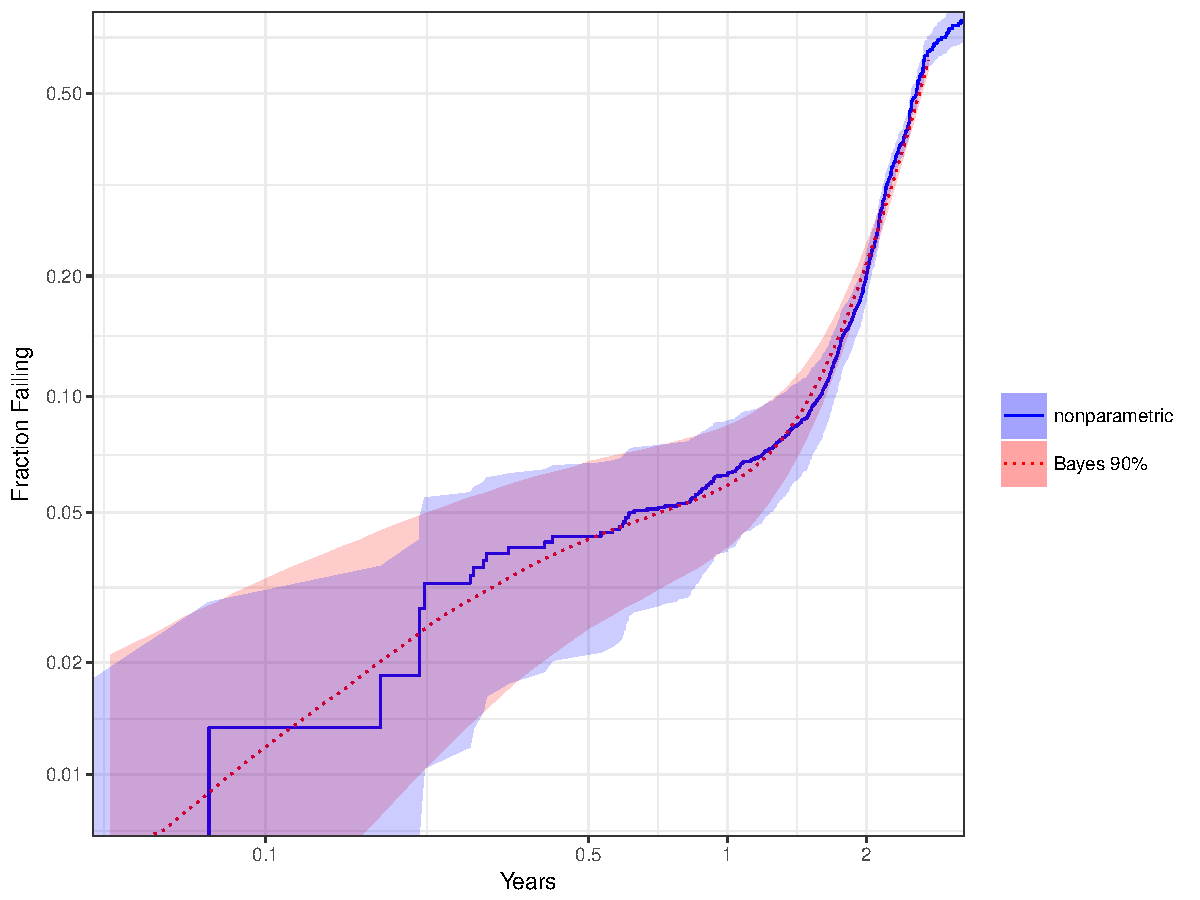
\includegraphics[width=.9\textwidth]{fig/drive14cred.pdf}
  \caption{Estimated GLFP for drive-model 14 plotted on Weibull paper.  Dashed line corresponds to the median of the posterior draws.  Solid blue line is a non-parametric Kaplan-Meier estimator.  Credible 90\% bands are in red.  Greenwood non-parametric error bands are in blue.}
  \label{fig1}
\end{figure}


\section{Hierarchical GLFP model}
\label{sec:Hierarchical GLFP model}

To borrow strength across different product populations, we can either share parameters across products, or model the product specific parameters hierarchically, allowing the data to inform the hyperparameters. For the second option, we model the scales, $\sigma_j$, quantiles, $t_{p_j,d,j}$, and proportions, $\pi_d$, of the component distributions as follows:

$$\sigma_{d,1} \ind \op{Lognormal} \left( \eta_{\sigma,1}, \tau^2_{\sigma,1} \right) \mbox{ for } d=1,\ldots,D$$
$$\sigma_{d,2} \ind \op{Truncated-Lognormal} \left( \eta_{\sigma,2}, \tau^2_{\sigma,2} , 0, 1 \right) \mbox{ for } d=1,\ldots,D$$
$$t_{p_j,d,j} \equiv \mu_{d,j} + \sigma_{d,j}\,\Phi^{-1}(p_j)  \ind \op{Normal} \left(\eta_{t_{p_j},j}, \tau^2_{t_{p_j},j}\right) \mbox{ for } j=1,2\; d=1,\ldots,D$$

$$\op{logit} \pi_d \ind \op{N}(\eta_\pi, \tau_\pi) \mbox{ for } d=1,\ldots,D.$$

Here, $\Phi^{-1}$ is the quantile function of the standard log-Weibull distribution. We truncate $\sigma_{d,2}$ at $1$, appealing to the logic that, by nature, wearout produces an increasing hazard function. The decision to parameterize in terms of a quantile other than the log-location parameter, $\mu = t_{0.632}$, is that lifetime data often features heavy right-censoring where inferences about the location parameter are extrapolations beyond the range of the data. %For this data we selected $p_1=0.5,\mbox{ (the median), and } p_2 = 0.2$.

We consider the models with the following set of restrictions (from most to least restrictive):

\begin{enumerate}
\item $\pi_{d} = \pi,\quad \mu_{d1} = \mu_1,\quad \sigma_{1}=\sigma_1,\quad \mu_{d2} = \mu_2,\quad \sigma_{d2} = \sigma_2$
\item $\pi_{d} = \pi,\quad \mu_{d1} = \mu_1,\quad \sigma_{d1}=\sigma_1,\quad \sigma_{d2} = \sigma_2$
\item $\pi_{d} = \pi,\quad \mu_{d1} = \mu_1,\quad \sigma_{d1}=\sigma_1$
\item $\mu_{d1} = \mu_1,\quad \sigma_{d1}=\sigma_1$
\end{enumerate}

The set of model specifications were chosen based data, interpretation of the model, as well as estimation considerations.  Product specific parameters for the the wearout failure mode $(\mu_{d2},\sigma_{d2})$, and the proportion defective $(\pi_d)$, are considered as a means to account for heterogeneity across brands in the right tails of the failure distribution.  Going from a common model for all product brands and gradually increasing the complexity of the model, we end up at Model 4.  Model 4 allows for the probability of infant mortality as well as the shape and scale parameters for the 2nd failure mode to vary by product.

For all of the models we consider, the parameters for the infant mortality failure mode are held in common across products.  We found that there was often insufficient information to model these parameters hierarchically.  Moreover, assuming a common distribution for infant mortality provides a meaningful interpretation and comparison of $\pi_i$ and $\pi_j$ ($i \neq j$). 


\section{Data analysis}
\label{sec:Data analysis}
\subsection{Data}
\label{sec:Data}
Backblaze is a company that offers cloud backup storage to protect against data loss.  Since 2013 it has been collecting data on hard drives operating at its facility.  The purpose is to provide consumers and businesses with reliability information on different hard drive-models.  The hard drives continuously spin in controlled storage pods.  Drives are run until failure.  When a hard drive fails it is permanently removed and replaced.  In addition, the number of storage pods is increasing as Backblaze adds to its storage capacity.  Every quarter Backblaze makes its data publicly available through their website \cite{backblaze}. In addition, Backblaze publishes summary statistics of the different hard drive-models currently operating.  No other analysis or modeling of the failure data is provided.  Backblaze does, however, encourage others to further analyze its data. 

As of the first quarter of 2016, Backblaze was collecting and reporting data on 63 different drive-models.  Some drive-models have been running since 2013 or before, while others were added at a later date.  Data have been reported on 75,297 different hard drives that are or where in operation.  The distribution of drives by drive-model varies: some drive-models have only have a service record for a single drive whereas the maximum number of daily service records for a single drive model is 35,860.  Figure \ref{fig1} shows the distribution of total number of failures and total observed running time for drive-models with at least 3 failures.  For model identification, a minimum of three failures was the criterion for hard drive brands to be included in our analyses.  

\begin{figure}[H]
  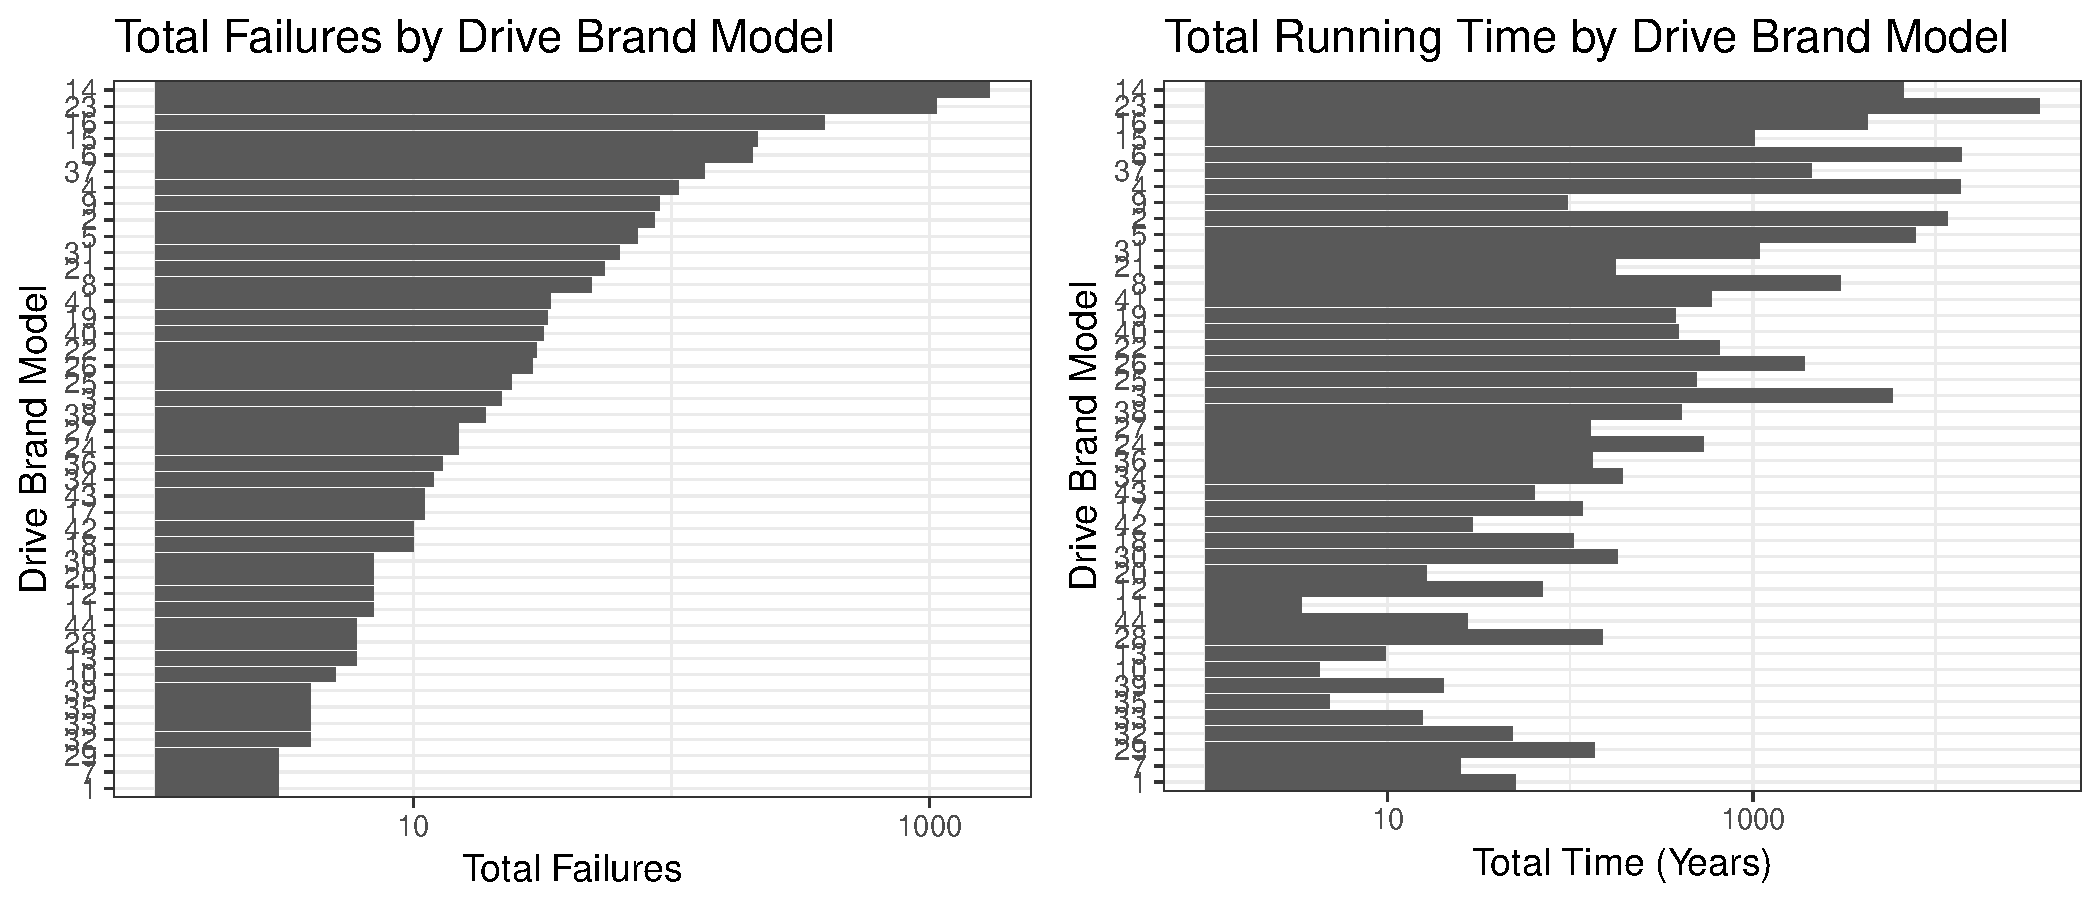
\includegraphics[width=.9\textwidth]{fig/data-sum.pdf}
  \caption{Left: Total number of failures (log scale) for drive-models with at least 3 observed failures in the Backblaze data. Right: Total accumulated time in operation (log scale) for each of the drive-models in the Backblaze data.  The plots are sorted based on the total number of failures on the left.}
  \label{fig1}
\end{figure}


Probability plotting is a simple method to assess the adequacy of (log)location-scale families of probability models to the data.  Identifying whether failure data are consistent with a specific family of distributions is difficult to do by examining a histogram or other density estimate.  By properly transforming the axes of a plot of an empirical estimate of fraction failing as a function of time with simultaneous confidence bands provides a graphical test for distributional goodness of fit.  

Applying this method to the hard drive data, we start with a non-parametric estimate of the empirical cdf for each drive-model using the Kaplan-Meier estimator
\cite{kaplan}.  With left truncation, however, the standard Kaplan-Meier estimator for drive-model $d$, denoted by
$\widehat{F_d(t)}_{KM}$, is conditional on survival up to
$t_{d,\text{min}}^L$, the shortest reported running time of all units
of drive-model $d$ for which records are available. To produce
unconditional estimates, we adapt the adjustment method outlined by
Turnbull, and given in more detail by Meeker and Escobar
\cite{turnbull,meeker}.  For each drive-model we select
$t_{d,\text{min}}^L$, the smallest left truncated time in the sample.
By sampling from the full posterior distribution, since
$\Pr(T>t_{d,\text{min}}^L|\theta_d)$ (the probability a hard drive has
survived up to $t_{d,\text{min}}^L$) is a function of the model
parameters, we can easily compute its posterior median,
$\widehat{A}_{\text{med}} = \widehat{Pr}(T>t_{d,\text{min}}^L|\theta_d)$. We compute the adjusted estimate by

$$\widehat{F(t)}_{KMadj} = \widehat{A}_{\text{med}} + \left(1 - \widehat{A}_{\text{med}}\right)\widehat{F_d(t)}_{KM},\; t>t_{d,\text{min}}^L.$$

While this adjustment is negligible for the majority of drive-models, five drive-models receive upward adjustments of greater than 5 percent and the estimated time to failure distribution of one drive-model (30) was adjusted by nearly 16 percent, in part because the shortest truncation time for all observed units was approx. 2.3 years.


In Figure 2 we plot the Kaplan-Meier adjusted cdf for drive-model 14 on Weibull paper.  Drive-model 14 had the most observed failures of all the brands.  Each point on the plot corresponds to an observed failure.  Censored drives are not plotted.  Standard error bands are calculated using Greenwood's method \cite{green}.  As mentioned in the introduction, the population of hard drives exhibits two primary failure modes.  One mode is a result of manufacturing defects, which cause early failures, known as infant mortality.  The second mode is non-defective hard drives that eventually fail due to wearout.   Evidence of at least two failure modes is seen in the Kaplan Meier plot with a kink occurring between 8000 and 20,000 hours.  Therefore, fitting a single Weibull model is not flexible enough to model the failure distribution.

\begin{figure}[H]
\centering
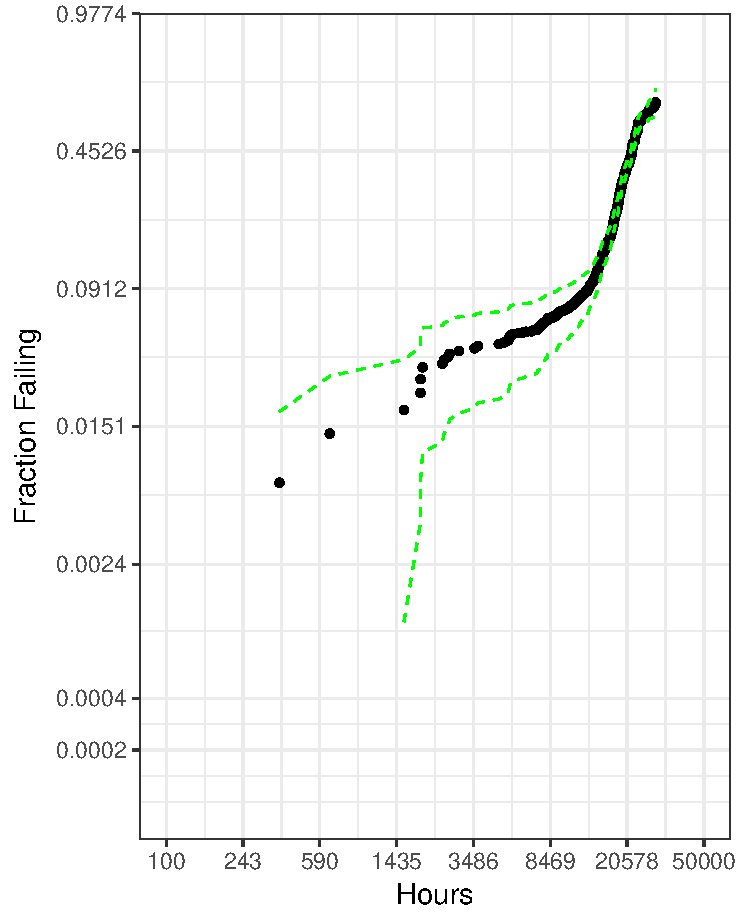
\includegraphics[width=.5\textwidth]{fig/mod14-KM-adj}
\caption{Truncated Adjusted Kaplan-Meier plot showing nonparametric estimate of fraction failing for drive-model 14.  Dashed lines are Greenwood standard errors.  Plotted on Weibull paper.}
\end{figure}


\subsection{Prior Distributions}
\label{sec:Prior Distributions}
To complete the full probability model, we need to select prior distributions for the parameters governing the hierarchical model. We select proper priors to ensure a proper posterior.

For models 1-4, different sets of restrictions required different prior specifications, which were assigned as follows:

\begin{enumerate}
\item This model constrains all drive-models to the same failure distribution. For this ``reduced" model we assume the same priors as in Example 1.

\item We allow $t_{pd}$ to vary by drive-model. To help with model identifiably, we tighten the priors on the defective mode:
$$ \mbox{logit}^{-1}\pi \sim \op{Normal}(-3,1),\quad \sigma_1 \sim \op{Lognormal}(0, 1), \quad t_{p1} \sim \op{Normal}(7,2),$$
implying now a prior $90\%$ probability that $\sigma_1$ is between $0.19$ and $5.18$ and $t_{0.5,1}$ between $3.7$ and $10.3$, which, translating from the log-scale, is equivalent to an interval from 1.5 days to 3.4 years.

\item $\sigma_{d2}$ is allowed to vary. Priors for constrained parameters are the same as for model 2.

\item $\pi_d$ varies. Priors for constrained parameters are the same as for model 2.

\end{enumerate}

For the scale hyper-parameters we follow the recommendations of \citet{gelman2014bayesian} and use half-Cauchy priors. As for the location hyper-parameters, we select weakly informative priors consistent with our prior information on hard-drives. The prior for $\eta_\pi$ puts 95\% of prior mass on the interval $(0.006, 0.27)$ for the median proportion defective (What justification? Should maybe be lower.) For $\eta_{\sigma, 2}$, $95\%$ of prior mass is on values greater than $0.037$. Since $\sigma_d$ is the reciprocal of the Weibull shape parameter, this corresponds roughly to an assumption that the median Weibull shape parameter is less than $1/0.037 = 27$. The prior for $\eta_{t_{p_2},2}$ implies that the median 20th percentile for non-defective units is less than greater than 3 days and less than 24 years.

\begin{align*}
  \eta_{\pi} & \sim \op{Normal}(-3, 1)\\
  \tau_{\pi} & \sim \op{Cauchy}^+(0, 1)\\
  \eta_{\sigma ,2} & \sim \op{Normal}(0, 2)\\
  \tau_{\sigma ,2} & \sim \op{Cauchy}^+(0, 1)\\
  \eta_{t_{.2_2},2} & \sim \op{Normal}(9, 2)\\
  \tau_{t_{.2_2},2} & \sim \op{Cauchy}^+(0, 1)
 \end{align*} 

\subsection{Computation}
\label{sec:Computation}
Each model was fit using the {\tt
  rstan}\cite{rstan} package in {\tt R} \cite{r}, which implements a variant of Hamiltonian Monte Carlo (HMC)
\cite{betancourt}. Multiple chain were run for 1500 iterations after 1500 warmup iterations. Convergence was assessed by examining posterior
plots and checking that potential scale reduction factors (Rhat) \cite{gelman2014bayesian} were less than $1.1$. Four chains were run for Models 1,2 and 3 and 16 chains were run for Model 4.



\subsection{Model Comparisons}
\label{sec:Model Comparisons}
The right side of Figure \ref{fig2} shows that the set of estimated failure curves for all four models that we fit. The upper left panel shows the estimated failure curve fit to all data ignoring drive-model as a factor (Model 1). The upper left plot, which represents Model 2, demonstrates that there is appreciable differentiation between drive-models; note that, because the scale parameter, $\tau_{t_{p2}}$ is learned hierarchically from the data, we can ascertain that there is evidence in the data that this variability is real.

The lower left panel, representing Model 3, suggests differing shape parameters in the wearout failure mode which means that the ranking of drive-models with respect to fraction failing differs over time.

Finally, the lower right panel, corresponding to Model 4, shows that, by allowing $\pi_d$ to vary by drive-model, there is greater variability in the early rate of failure and, for some drive-models, the forecasted fraction failing is adjusted downward. 

\begin{figure}[H]
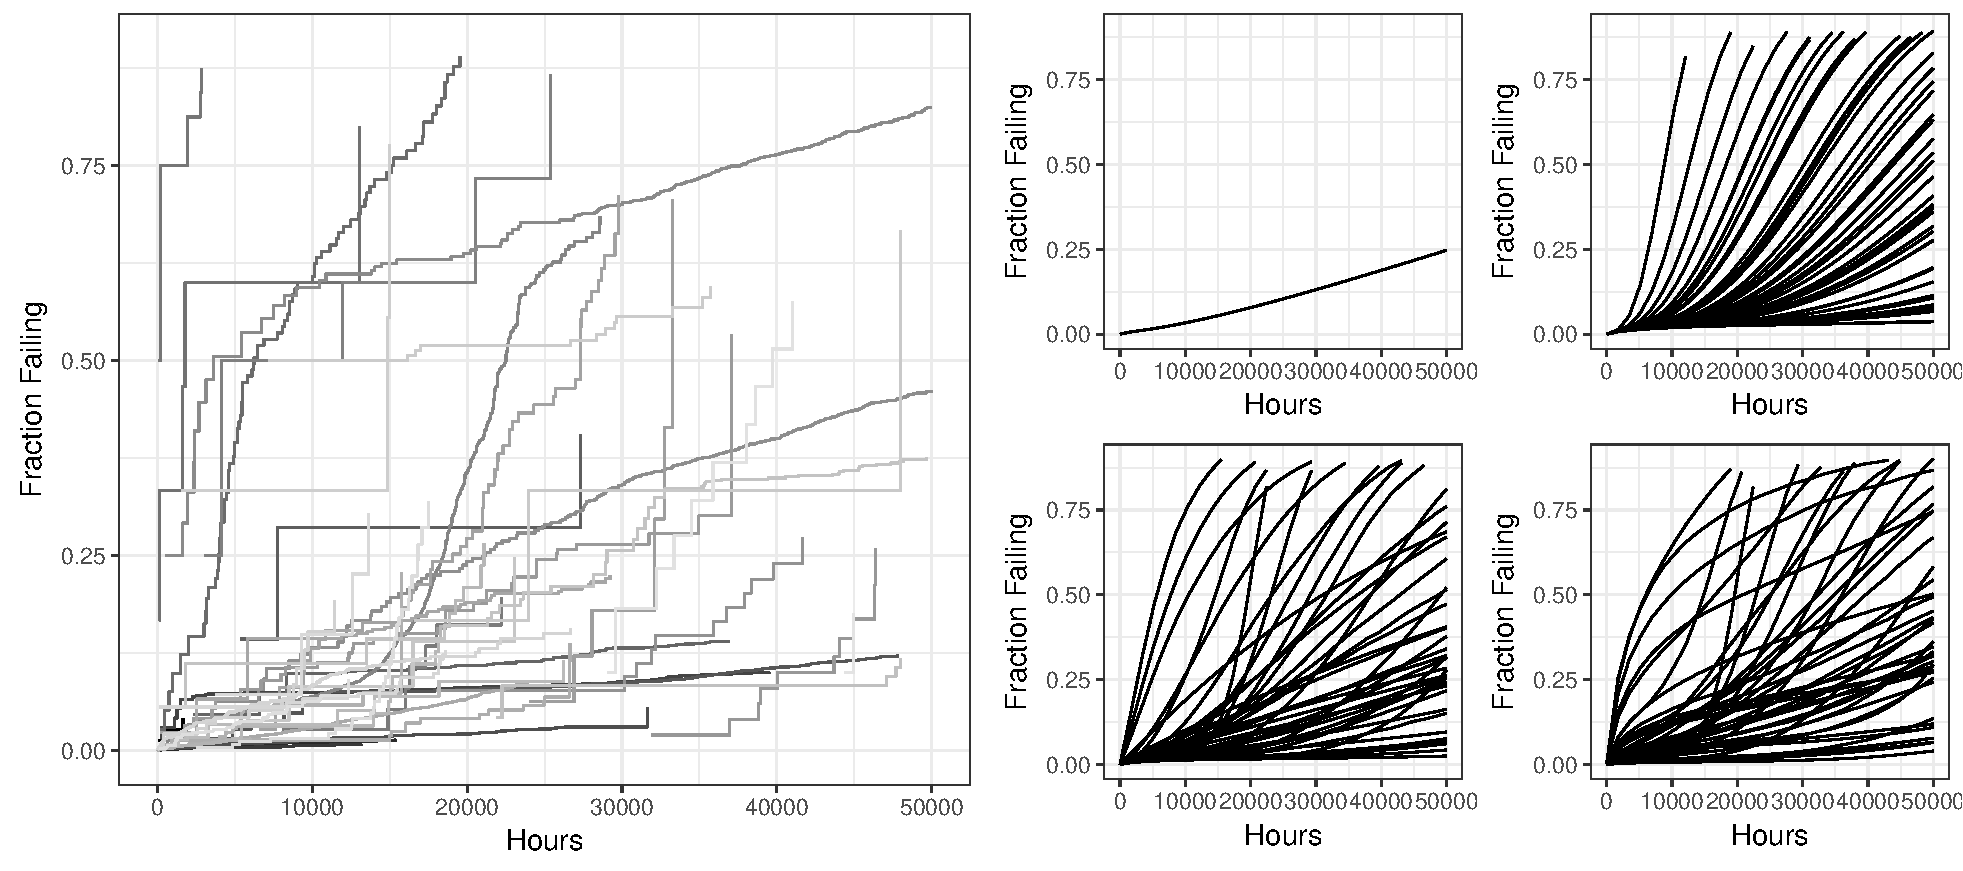
\includegraphics[width=\textwidth]{fig/heterogeneity-compare-preliminary}
\caption{Left: Kaplan-Meier estimates of the time to failure for each of the drive-models in the Backblaze data. Right: Pointwise posterior median time to failure curves for Models 1-4, ordered left to right, top to bottom.}
\label{fig2}
\end{figure}

We can also compare the model fits for each drive-model individually.  Using the set of parameters that maximize the posterior log probability, we examine the GLFP cdf for each of the 4 model specifications.  The GLFP fit for drive-models 2, 9, 14, and 40 are presented in Figure 4.  The black step functions again corresponds to the adjusted non-parametric estimates.  As model complexity increases, the GLFP curves become more flexible and are better able to fit the observed failure data.  All of the GLFP models appear to overestimate the proportion of failed hard drives for drive-model 2, but Model 4 agrees best with the nonparametric estimate.  For drive-model 14, Models 1-3 underestimate the proportion of drives failing, and for drive-model 40, they slightly overestimate the data.  Conversely, Model 4 follows the observed failures quite closely--accurately capturing failures at the lower and upper ends of the distribution.  The difference in accuracy between Models 3 and 4 are and Models 1 and 2 are visually quite apparent.  Differentiating between Model 3 and 4 is less clear; for instance, the fits from Model 3 and 4 line almost exactly on top of each other for drive-model 40.
\begin{figure}[H]
    \centering
   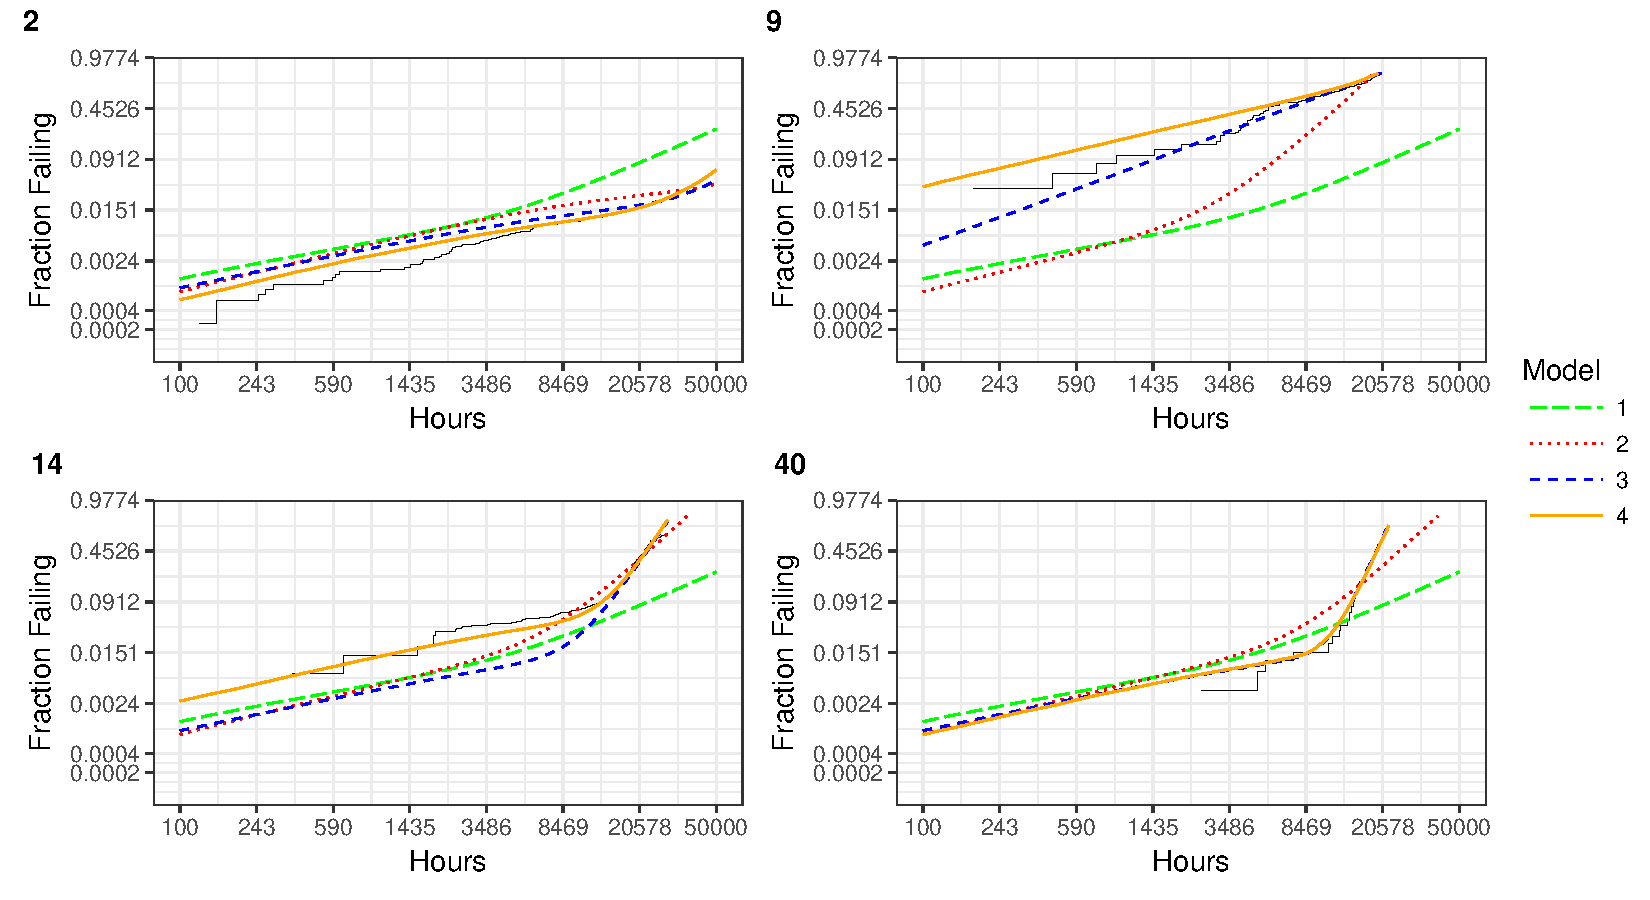
\includegraphics[width=\textwidth]{fig/mod_compare_legend}
		\caption{Estimated GLFP for 4 drive-models plotted on Weibull paper.  The solid step function is the truncated adjusted Kaplan-Meier points.  \label{fig:first}} 
\end{figure}


To statistically compare the GLFP Models, we estimated the predictive accuracy of the 4 different models using an approximate leave-one-out cross validation (LOO) method.  As outlined in Vehtari et. al, the predictive accuracy from a fitted Bayesian model can be estimated simply with posterior draws of the model parameters rather than re-fitting the model with different data sets \cite{vehtari}.  For each observation, $i$, the log point-wise predictive density is calculated over the full set of posterior samples with data point $i$ removed.  The final expected log point-wise predictive density (elpd) is the sum over all observations (elpd $=\sum{\log p(y_i|y_{-i})}$).  We computed the elpd for all 4 models using the R package loo \cite{loo}.  When $n$ is large, the distribution of the elpd is approximately normal and different models can be compared statistically.  We calculated the difference in expected predictive accuracy for Model 4 vs 3, Model 3 vs 2, and Model 2 vs 1, as well as the standard error of the difference (Table 1).  As the model complexity increased, the expected predictive accuracy improved.  Of all the models, Model 4 had the best predictive accuracy and was significantly better than the other 3 models.

\begin{table}[H]
\centering
\begin{tabular}{rrrrrrr}
  \hline
 & ELPD \ & Difference in ELPD \ & SE of the Difference \\ 
  \hline
Model 4 & -13309.5 & 40.7 & 11.3 \\ 
Model 3 & -13350.2 & 458.8 & 31.0  \\ 
Model 2 & -13809.0 & 3674.6 & 96.2 \\ 
Model 1 & -17483.6  \\ 
   \hline
\end{tabular}
\caption{Expected Log Pointwise Predictive Density (ELPD) for each model specification.  Each model is compared to the more parsimonious model below.  The estimated difference of expected leave-one-out prediction errors between the two models, as well as the standard error of the difference, is also presented.}
\label{table:1}
\end{table}


\subsection{Drive-model Comparisons}
\label{sec:Drive-model Comparisons}
We consider the problem of ranking drive-models. From a
business perspective, it is clear
that we should prefer the drive-models which will provide more years
of service. For ease of exposition, we will assume that the purchase
price of a hard-drive is the same across drive-models.

There are two sources of variation at play; the
posterior uncertainty in the parameters, which largely depends on the
sample size, and the uncertainty in future
observations conditional on the parameters. The {\em posterior
  predictive} distribution incorporates both sources.
\begin{equation*}
  p(t_{d,new}|t) = \int p(t_{d,new}|\theta_d) p(\theta_d|t) \, d\theta_d
\end{equation*}

We can sample from this distribution by drawing $t_{d,new}^{(s)}$ from
$\operatorname{GLFP}(\pi_d^{(s)},
\mu_1^{(s)},\sigma_1^{(s)},\mu_{2,d}^{(s)},\sigma_{2,d}^{(s)})$, for
$s=1,...,S$, using the saved posterior draws for the model
parameters. The expected time-to-failure (TTF) for drive-model $d$ can be estimated by
$$\frac{1}{S} \sum_{s=1}^{S} t_{d,new}^{(s)}.$$

While TTF is clearly important, due to the
anticipation of advancements in technology, we can expect that the
relative value of computer hardware will depreciate rather quickly. To account
for this depreciation, rather than using TTF as the metric for drive-model comparison, we use the value at replacement. The IRS considers
computer hardware to be ``5-year'' equipment\cite{f4562}. Using``the declining
balance method'' the rate of depreciation is 40\% per year.

Let $L(t) = e^{-.4t}$ represent the value at the time of failure
relative to a new unit. We can rank the drive-models by 
$$\op{E}(L(t_{d,new})|t))\approx \frac{1}{S} \sum_{s=1}^{S} L(t_{d,new}^{(s)}).$$


We can also use the posterior draws to compute quantiles of interest, which in reliability applications is typically more informative than a central measure of tendency.  On the left panel of Figure 5 we plot $t_{0.10}$, the .10 quantile (i.e., the amount of time it takes for 10\% of hard drives to fail), for all drive-models. The best six drive-models ranked by TTF are also the drive-models with the longest time to $t_{0.10}$.  Drive-models 5, 2, 4, and 3 seem to really stick out as the most reliable as there is a larger gap separating them from the rest of the group.  Another interesting feature to compare is $\pi$, the proportion failing due to infant mortality.  One the right panel of Figure 5 are the posterior credible intervals of $\pi$ for each drive-model.  The plot is again sorted according to $t_{0.10}$ so it can be compared to the left hand side.  While for many of the drive-models the ordinal ranking is the same as on the left, there are some drive-model comparisons, for example 23 and 18, that differ in ranking if compared using $t_{0.10}$ or $\pi$.  Depending on a user's application or the hard drive warranty length, using the $\pi$'s as a comparison tool may be a relevant parameter of interest.   
 
\begin{figure}[H]
  \centering
  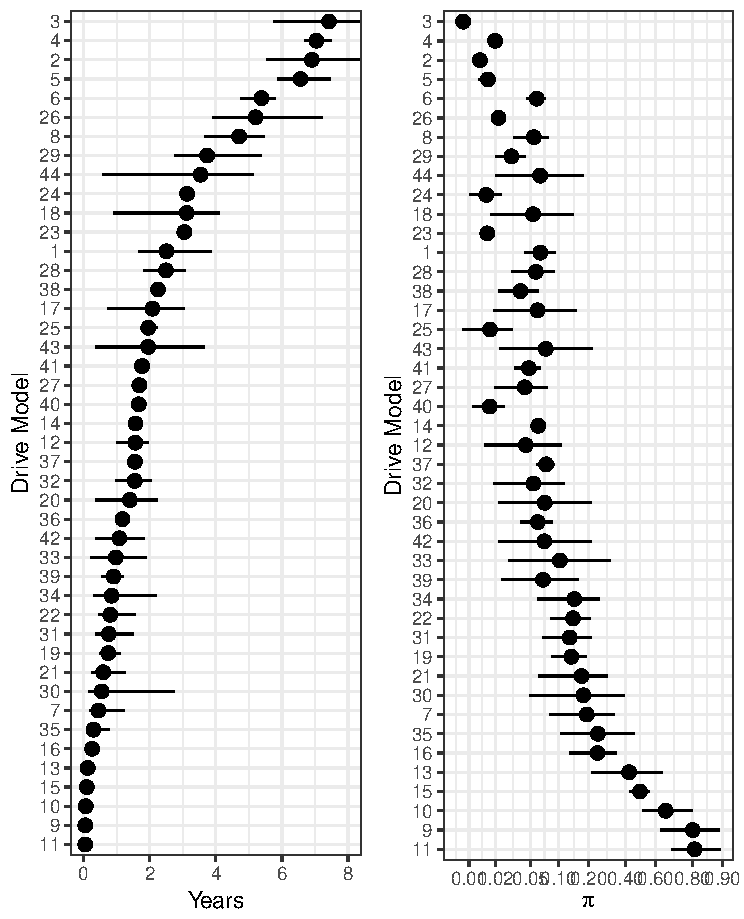
\includegraphics[width=\textwidth]{fig/b10andpi}
  \caption{Left: 50\% credible intervals for  $t_{0.10}$ (time in years till 10\% of the drives fail). Right: 50\% credible intervals for $\pi$ plotted on the logit scale.  Both plots are sorted based on the median value of $t_{0.10}$.}
  \label{fig4}
\end{figure}

\begin{figure}[H]
  \centering
  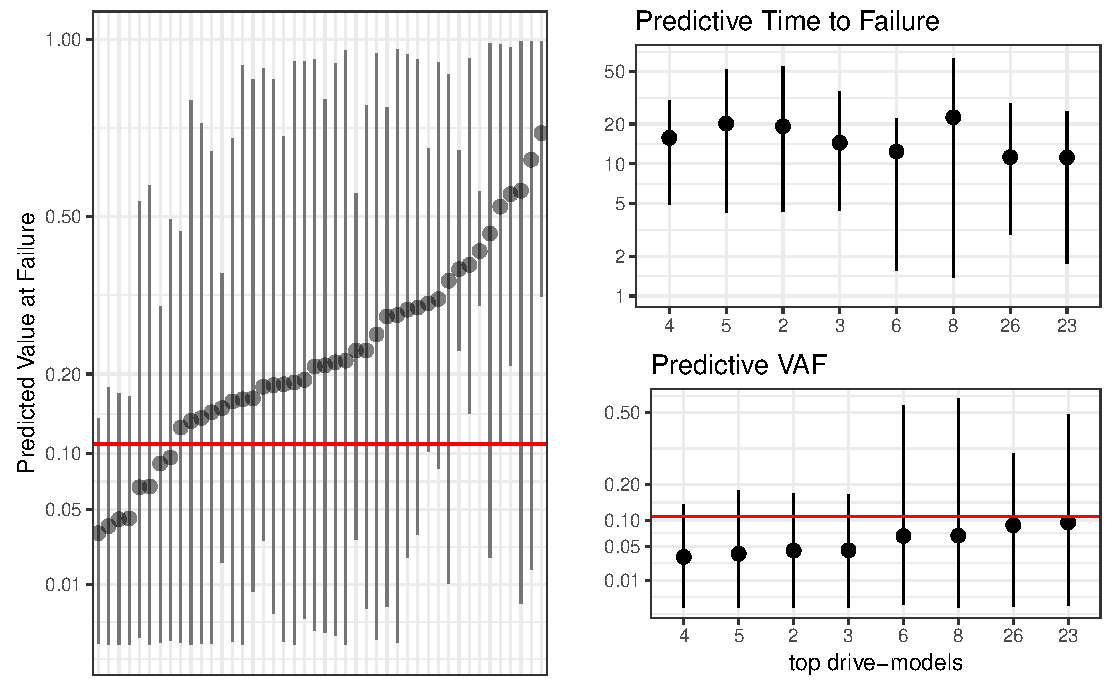
\includegraphics[width=.8\textwidth]{fig/dm-eval}
  \caption{Left: Posterior predictive relative value-at-loss for new
    unit, by drive-model. Right: TTF (top) and VAF based on 40\% annual depreciation (bottom), for best 11 drive-models.}
  \label{fig5}
\end{figure}


\section{Conclusions}
\label{sec:Conclusions}
We should point out some assumptions made in this analysis. First, we assume exchangability of units within drive-models. This assumption is due to our ignorance about the causes of failure and of potentially important covariates. If we had information about distinguishing characteristics of the two identified failure modes, then we should use this information. Also, there could be many environmental or human-related factors that impact lifetime, such as operating conditions associated with location in the data center, which are likely confounded with drive-model.

Second, it is probably true that many modes of failure occur and that the heterogeneity that we observe among drive models is due to different combinations of these. Our ignorance of the causes of failure leads us to approximate the main failure mode with a single drive-model specific Weibull distribution. Because of this, we suspect that our forecasts are too confident; especially for ``well-estimated" models, our uncertainty in the right tail of the distribution is probably too small. On the other hand, our model borrows strength across drive-models, including those with information about late failures. In addition, we suggest that using metrics for comparing drive-models that reduce the importance of the right tail of the distribution are appropriate for these data. With respect to decisions based on such metrics, we believe the assumptions in the previous paragraph to be the most critical. Those issues are typical to observational data such as these.

Consumers of high-tech manufactured goods usually lack the expertise to perform a failure analysis to determine the cause of failure. The ability to fit marginal models, such as GLFP, can allow investigators to answer many pertinent questions while still appropriately accounting for uncertainty and avoiding substantial model bias.

Advances in technology have made computationally intensive Bayesian methods for fitting hierarchical models feasible in practice. Hierarchical modeling can be an effective way to regularize a large number of models fits by borrowing information. Because all the data contribute some information about the global parameters, it is often sufficient to use weakly informative priors on the global parameters, making the resulting shrinkage data dependent. Using samples from the full joint posterior avoids the need for potential problematic asymptotic approximations.

Analysis using HMC is accessible to practitioners by Stan. HMC has been shown to be very efficient in effective samples per iteration because its joint updating scheme.


\pagebreak

\begin{center}
{\large\bf SUPPLEMENTARY MATERIAL}
\end{center}

\begin{description}

\item Put R Stan code here

\end{description}

\begin{appendix}
\scriptsize
\begin{verbatim}
functions {
  real sev_logpdf(real y, real mu, real sigma){
    real z;
    z = (y - mu) / sigma;
    return -log(sigma) + z - exp(z);
  }
  
  real sev_logccdf(real y, real mu, real sigma){
    return -exp((y - mu) / sigma);
  }
  
  real sev_logcdf(real y, real mu, real sigma){
    return log1m_exp(-exp((y - mu) / sigma));
  }
}

data {
  int M;
  int N_obs;
  int N_cens;
  real endtime_obs[N_obs];
  real endtime_cens[N_cens];
  real starttime_obs[N_obs];
  real starttime_cens[N_cens];
  int<lower=1, upper=M> dm_obs[N_obs];
  int<lower=1, upper=M> dm_cens[N_cens];
  vector<lower=0, upper=1>[2] p; # quantiles to model
}
transformed data{
  vector[2] z_corr;
  for(i in 1:2)
    z_corr[i] = log(-1.0 * log1m(p[i])); # used to get location(mu) from quantile(t_p)
}
parameters{
  real log_tp1;
  real<lower=0> sigma1;
  real eta_tp2;
  real eta_s2;
  real eta_pi;
  real<lower=0> tau_tp2;
  real<lower=0> tau_s2;
  real<lower=0> tau_pi;
  vector[M] log_tp2_raw;
  real<lower=0, upper=1> sigma2[M];
  vector[M] logit_pi_raw;
}

transformed parameters{
  real mu1;
  vector[M] mu2;
  vector[M] log_pi;
  mu1 = log_tp1 - sigma1 * z_corr[1];
  for(m in 1:M){
    mu2[m] = (eta_tp2 + tau_tp2 * log_tp2_raw[m]) - (sigma2[m] * z_corr[2]);
  }
  for(m in 1:M)
    log_pi[m] = log_inv_logit(eta_pi + tau_pi * logit_pi_raw[m]);
}

model{
  real tmp[2];
  int m;
  real logpi;
  real mu_1;
  real mu_2;
  real sig_1;
  real sig_2;
  
  for(i in 1:N_obs){
    m = dm_obs[i];
    logpi = log_pi[m];
    mu_2 = mu2[m];
    sig_2 = sigma2[m];
    // numerator:   log( p * f1 * (1 - F2) + f2 * (1 - p * F1) )
    //            = log( exp(log(p) + log(f1) + log(1 - F2)) + exp(log(f2) + log(1 - exp(log(p) + log(F1)))) )
    tmp[1] = log_sum_exp(logpi + sev_logpdf(endtime_obs[i], mu1, sigma1) +
               sev_logccdf(endtime_obs[i], mu_2, sig_2),
               sev_logpdf( endtime_obs[i], mu_2, sig_2) + 
               log1m_exp(logpi + sev_logcdf(endtime_obs[i], mu1, sigma1)
               )
             );
    // denominator:  log((1 - p * F1) * (1 - F2))
    //            =  log(1 - p * F1) + log(1 - F2)
    tmp[2] = log1m_exp(logpi + sev_logcdf(starttime_obs[i], mu1, sigma1)) + 
             sev_logccdf(starttime_obs[i], mu_2, sig_2);
             
    target += tmp[1] - tmp[2];
  }
  
  for(i in 1:N_cens){
    m = dm_cens[i];
    logpi = log_pi[m];
    mu_2 = mu2[m];
    sig_2 = sigma2[m];
  
    // numerator:   log((1 - p * F1) * (1 - F2))
    //            =  log(1 - p * F1) + log(1 - F2)
    tmp[1] = log1m_exp(logpi + sev_logcdf(endtime_cens[i], mu1, sigma1)) + 
             sev_logccdf(endtime_cens[i], mu_2, sig_2);
    // denominator:  log((1 - p * F1) * (1 - F2))
    //            =  log(1 - p * F1) + log(1 - F2)
    tmp[2] = log1m_exp(logpi + sev_logcdf(starttime_cens[i], mu1, sigma1)) + 
             sev_logccdf(starttime_cens[i], mu_2, sig_2);
             
    target += tmp[1] - tmp[2];
  }
  
  log_tp1        ~ normal(7, 2);
  log_tp2_raw    ~ normal(0, 1);
  sigma1         ~ lognormal(0, 1);
  sigma2         ~ lognormal(eta_s2, tau_s2);
  logit_pi_raw   ~ normal(0, 1);
  eta_tp2       ~ normal(9, 2);
  eta_s2         ~ normal(0, 2);
  eta_pi         ~ normal(-3, 1);
  tau_tp2       ~ cauchy(0,1);
  tau_s2         ~ cauchy(0,1);
  tau_pi         ~ cauchy(0,1);
}

\end{verbatim}
\end{appendix}

\pagebreak

\bibliographystyle{plainnat}
\bibliography{sample}

\end{document}
